\documentclass[9pt]{beamer}

\usetheme{TUDo}



% Encoding je nach Compiler
\ifluatex
\usepackage[utf8]{luainputenc}
\else
\usepackage[utf8]{inputenc}
\usepackage[T1]{fontenc}
\fi


% Mathematik
\usepackage{amsmath}
\usepackage{amsfonts}
\usepackage{amssymb}
\usepackage{cancel}

%Links
\usepackage[]{hyperref}

%Float
\usepackage[]{float}

\renewcommand{\figurename}{Fig.}

%%%%%%%%%%%%%%%%%%%%%%%%%%%%%%%%%%%%%%%%%%%%%%%%%%%%%%%%%%%%%%%%%%%%%%%%%%%%%%%%
%%%%%-------------Hier Titel/Autor/Grafik/Lehrstuhl eintragen--------------%%%%%
%%%%%%%%%%%%%%%%%%%%%%%%%%%%%%%%%%%%%%%%%%%%%%%%%%%%%%%%%%%%%%%%%%%%%%%%%%%%%%%%

%Titel:
\title{Accessmail - an accessible E-Mail Client}
%Autor
\author{Simon Demming}
%Lehrstuhl/Fakultät
\institute[Department]{\par\smallskip\smallskip Department for Rehabilitation\\ Department for Computer Science}


\begin{document}

	\begin{frame}
		\setcounter{framenumber}{0}
	    \titlepage
	\end{frame}
	
	\begin{frame}
	    \frametitle{The team}
	    % Picture of Jonas
	    Jonas Langenberg \\
	    23 years\\
	    7th Semester BA Computer Science\\
	    % Picture of me
	    Simon Demming\\
	    22 years\\
	    6th Semester BA Computer Science\\
	    
	\end{frame}
	
	%Einführung
	\section{Introduction}
		
		\begin{frame}
			\frametitle{Introduction}
			
			Email as a very important communication platform used for
			\begin{itemize}
				\item Private communication
				\item Labour affairs
				\item Finances
				\item Entertainment
			\end{itemize}
		\end{frame}
		
		\begin{frame}
			\frametitle{Introduction}
			\begin{figure}
				\centering
				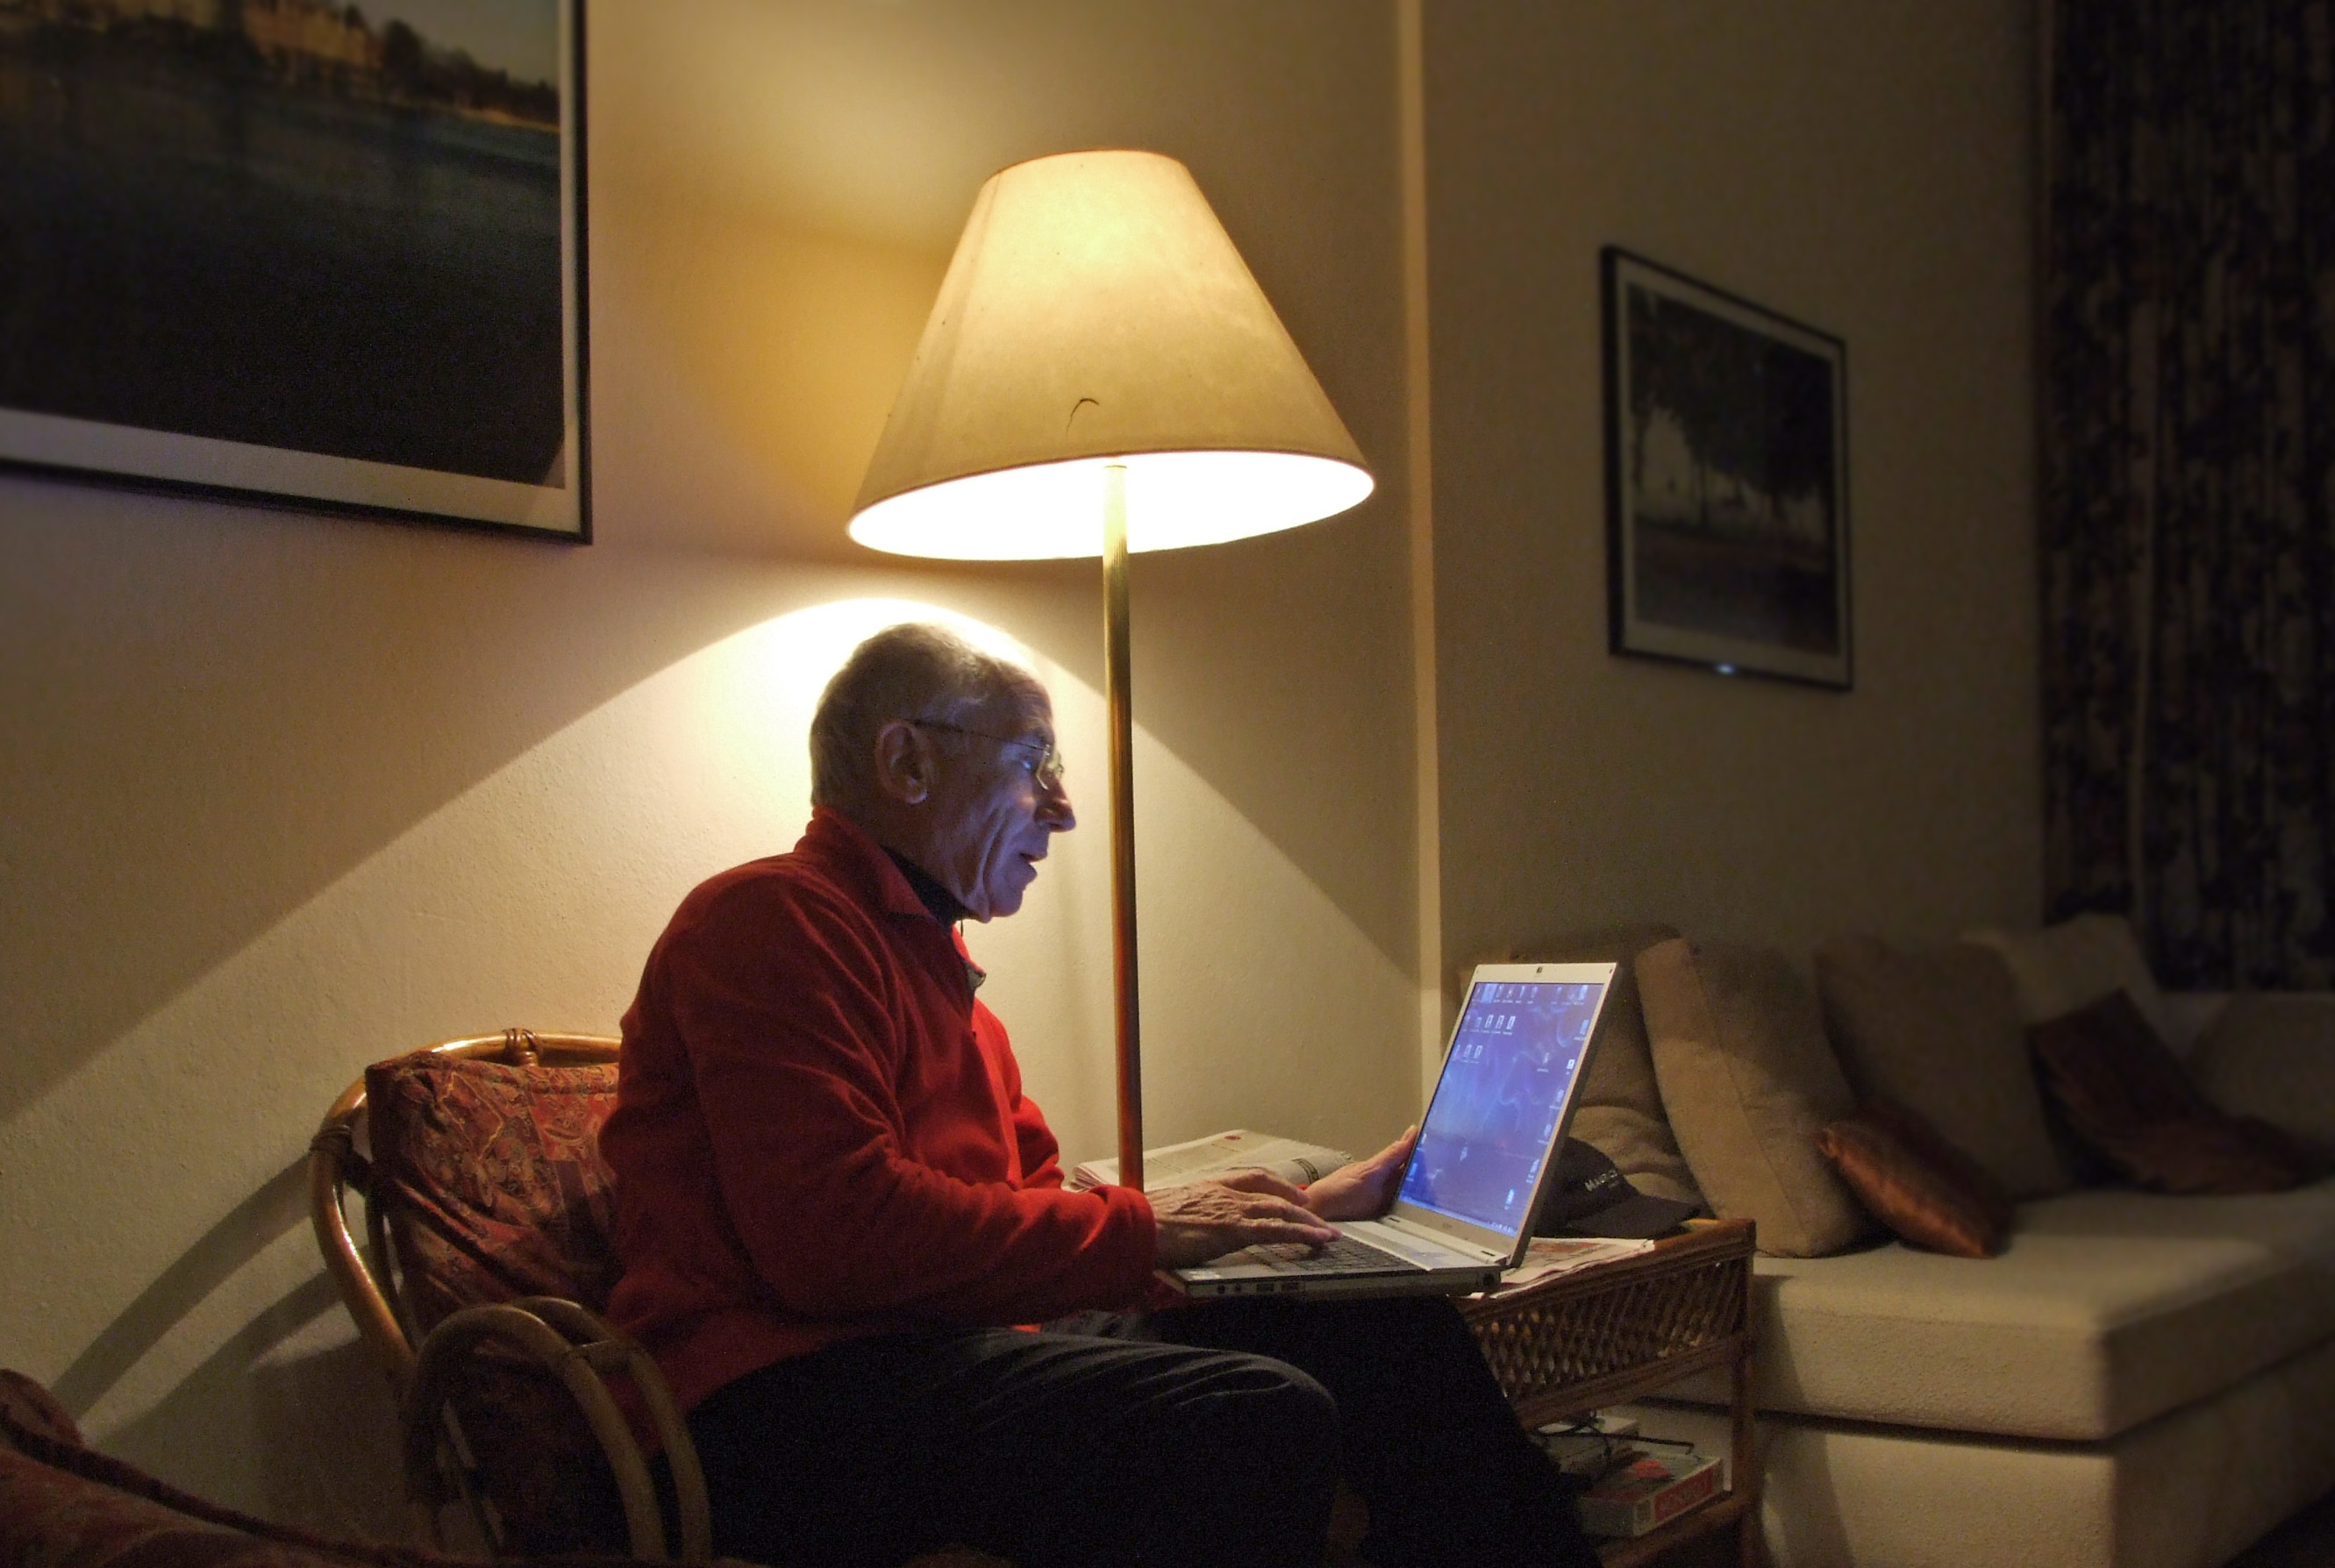
\includegraphics[scale=0.1]{Images/computersenior.jpg}
				%TODO add source "Rainer Sturm  / pixelio.de"
			\end{figure}
		\end{frame}
		
		\begin{frame}
			\frametitle{Email is not easy}
			\begin{figure}
				\centering
				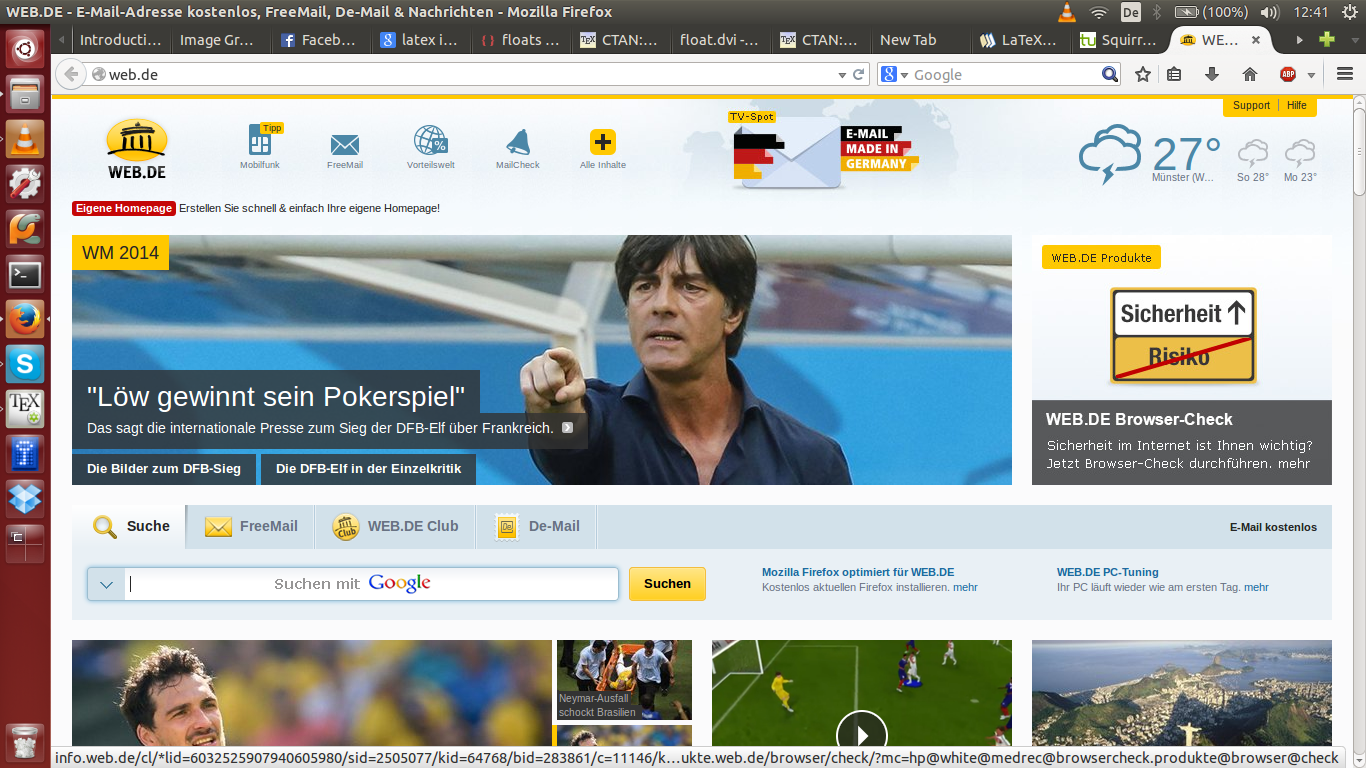
\includegraphics[scale=0.2]{Images/webstart.png}
			\end{figure}
		\end{frame}
		
		\begin{frame}
			\frametitle{Email is not easy}
			\begin{figure}
				\centering
				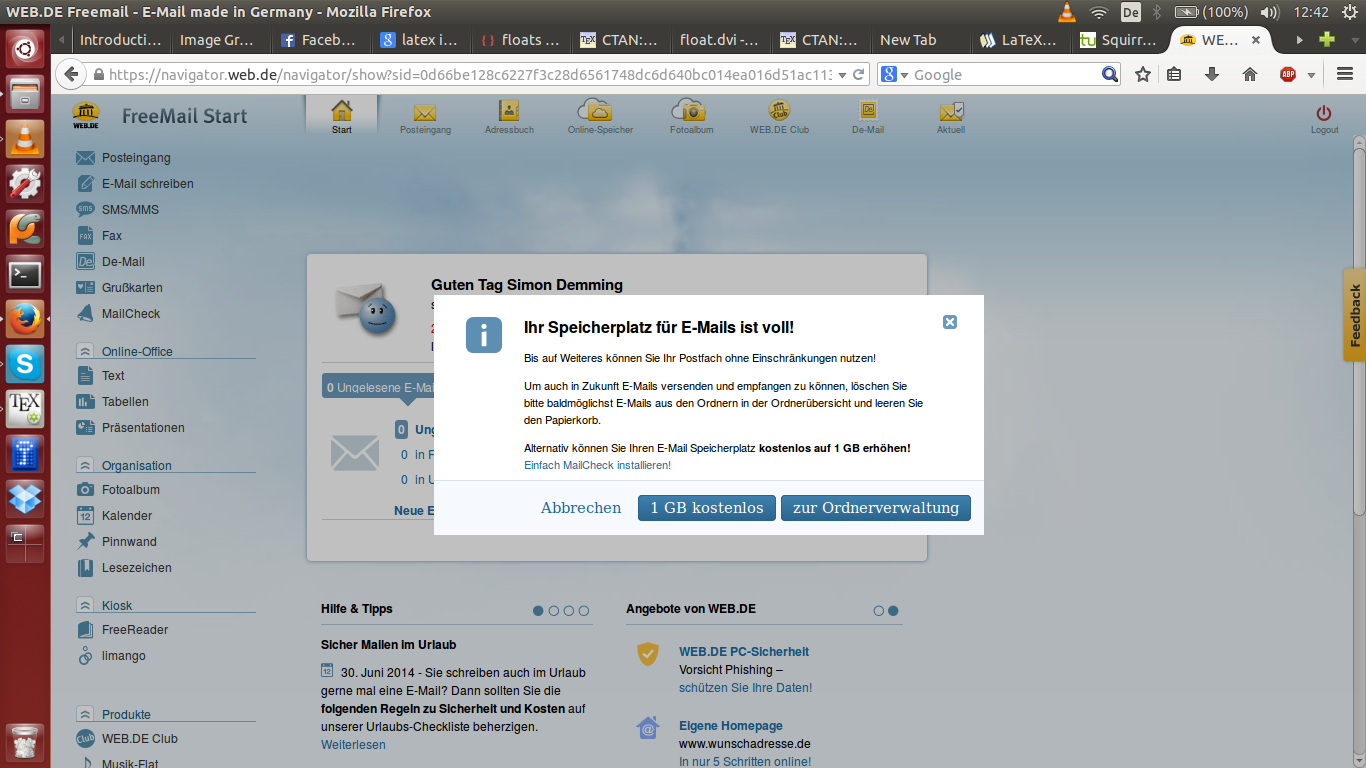
\includegraphics[scale=0.2]{Images/webstartmail.png}
			\end{figure}
		\end{frame}
		
		\begin{frame}
			\frametitle{Email is not easy}
			\begin{figure}
				\centering
				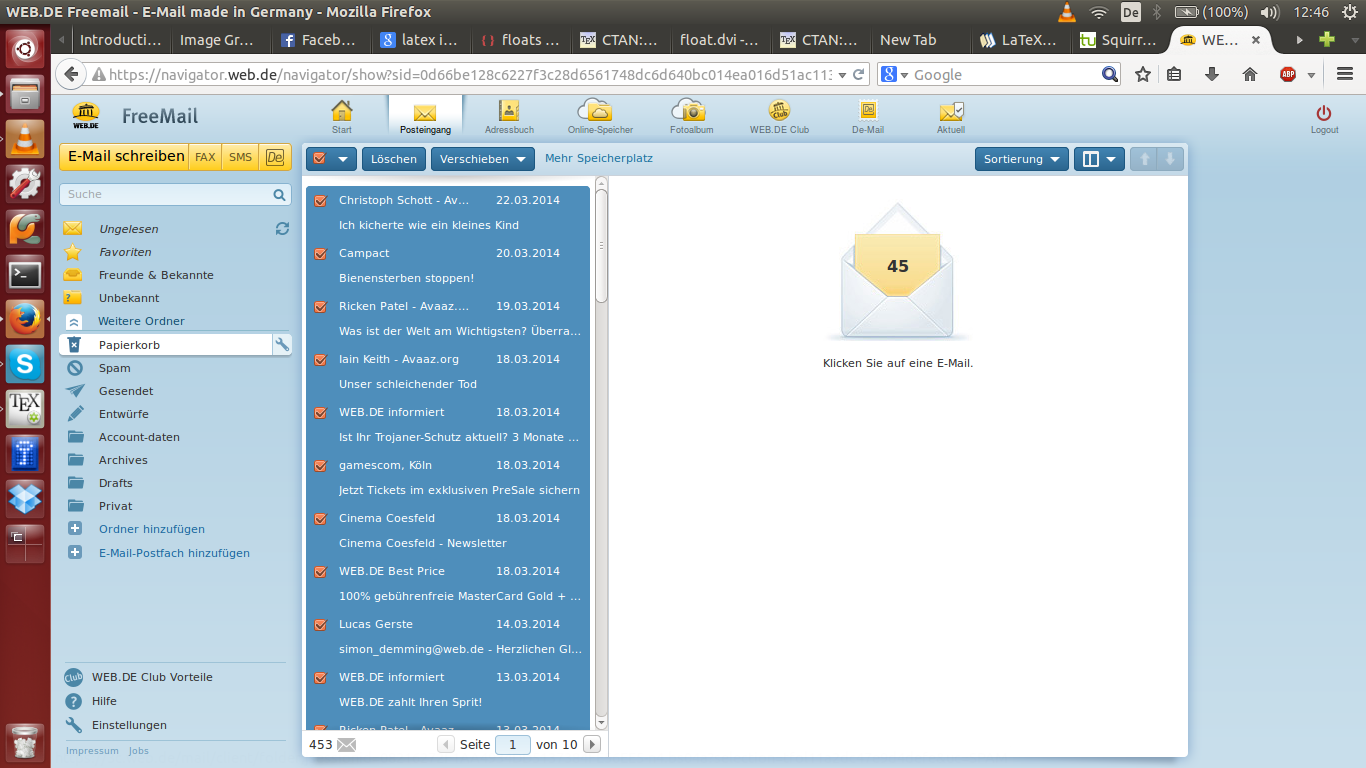
\includegraphics[scale=0.2]{Images/deletemailserror.png}
			\end{figure}
		\end{frame}
		
		\begin{frame}
			\frametitle{Email is not easy}
			\begin{figure}
				\centering
				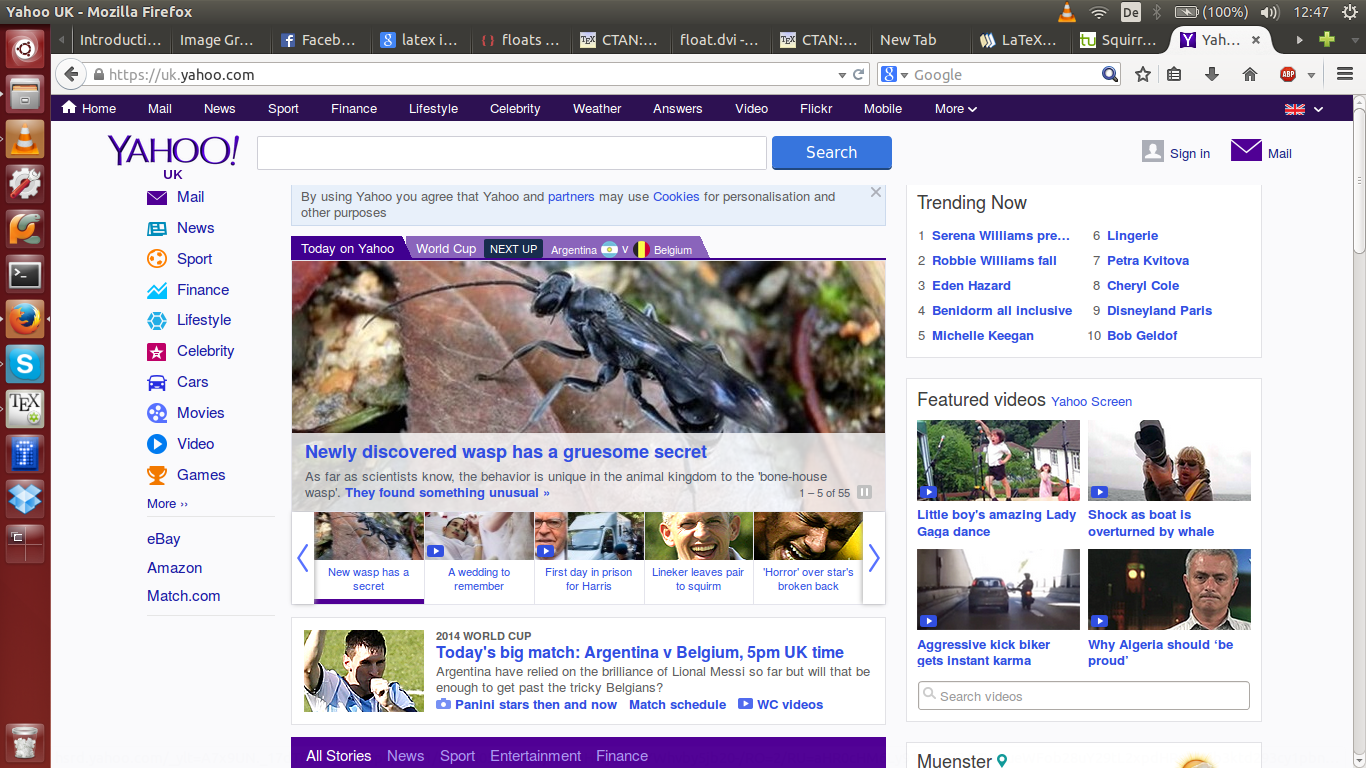
\includegraphics[scale=0.2]{Images/yahoostart.png}
			\end{figure}
		\end{frame}
	
	\section{Our Approach}
		\subsection{Preparations}
		
		\begin{frame}
			\frametitle{Preparations}
			\begin{figure}
				\centering
				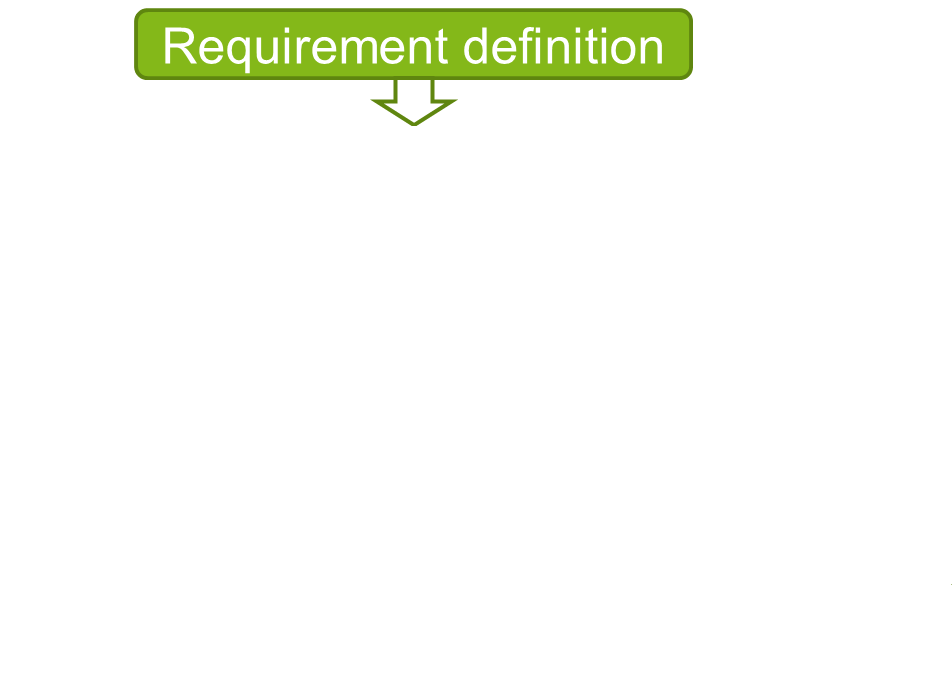
\includegraphics[scale=0.2]{Images/project_schedule_1.png}
			\end{figure}
		\end{frame}
		
		\begin{frame}
			\frametitle{Requirements}
			\begin{itemize}[<+->]
				\item Simple design\\
				$\rightarrow$ High usability
				\item High contrast\\
				$\rightarrow$ Good for visually impaired persons
				\item No distractions\\
				$\rightarrow$ High usability again
				\item Obvious pictographs\\
				$\rightarrow$ Good for persons with learning disabilities (and internationalisation)
				\item Foreseeable behaviour\\
				$\rightarrow$ No confusion
				\item Confirmations\\
				$\rightarrow$ No accidental deletions
			\end{itemize}
		\end{frame}
	
		\subsection{Software Design}
			\begin{frame}
				\frametitle{Software Design}
				\begin{figure}
					\centering
					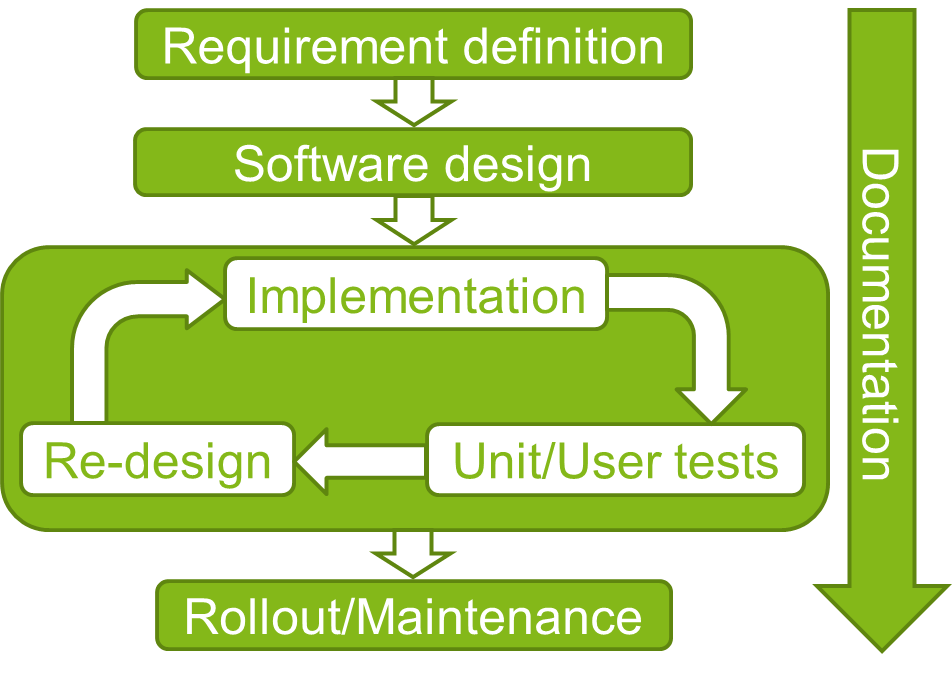
\includegraphics[scale=0.25]{Images/project_schedule_2.png}
				\end{figure}
			\end{frame}
			
		\subsection{Kivy Framework}
			\begin{frame}
				\frametitle{The Kivy Framework}
				\begin{itemize}
					\item Cross platform
					\item Business Friendly
					\item GPU Accelerated
				\end{itemize}
				
				\begin{figure}
					\centering				
					
\includegraphics[scale=0.3]{Images/kivy_logo.png}
					\caption{http://www.kivy.org/ - 02.July, 2014}
				\end{figure}
			\end{frame}
			
			\begin{frame}
				\frametitle{Kivy example}
				\begin{figure}
				\centering
				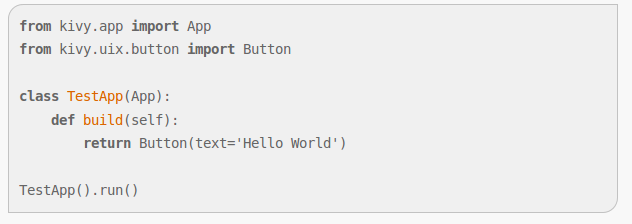
\includegraphics[scale=0.3]{Images/kivy_helloworld_code.png}
				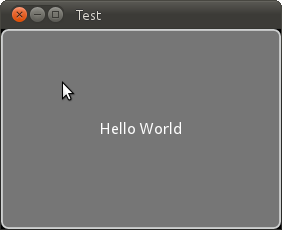
\includegraphics[scale=0.3]{Images/kivy_helloworld_result.png}
				\end{figure}
			\end{frame}
			
		\subsection{Packaging}
			\begin{frame}
				\frametitle{Packaging}
				\begin{figure}
					
\includegraphics[scale=1]{Images/pyinstaller_logo.png}
				\end{figure}
				\begin{itemize}
					\item PyInstaller - Packaging for Python
					\item Cross platform
					\item Challenges: Missing libraries, incomplete wrapping
				\end{itemize}
			\end{frame}
			
	\section{Testing routines}
		
		\begin{frame}
			\frametitle{Preparations}
			Aims:
			\begin{itemize}
				\item Finding bugs
				\item Test usability
				\item Get feedback on design
			\end{itemize}
			Material:
			\begin{itemize}
				\item The software packed for Windows
				\item The hardware
				\item A testing script
			\end{itemize}
		\end{frame}
		
		\begin{frame}
			\frametitle{The script}
			Automatically test the following functions:
			\begin{itemize}
				\item Create an email account
				\item Add a contact
				\item Write an email
				\item etc.
			\end{itemize}
		\end{frame}
		
		\begin{frame}
			\frametitle{Testing}
			\begin{figure}
				\centering
				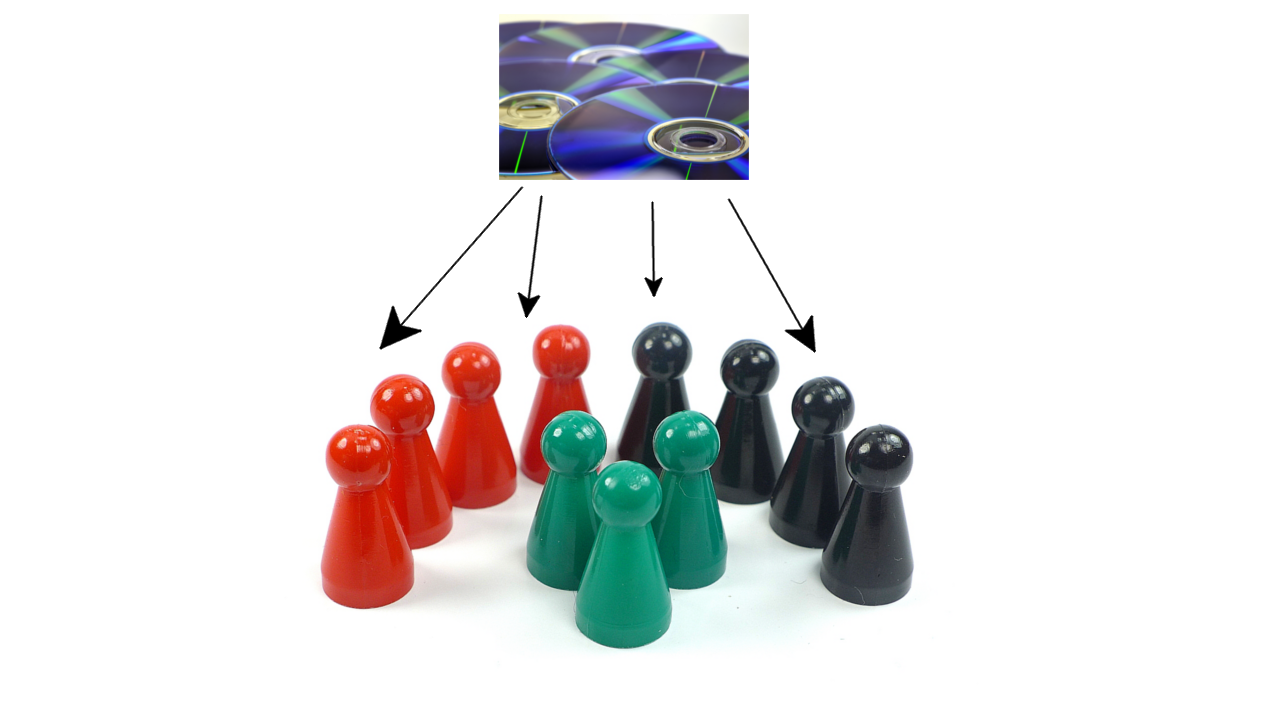
\includegraphics[scale=0.5]{Images/test_distribution.png}
			\end{figure}
		\end{frame}
		
		\begin{frame}
			\frametitle{Testing routines}
			\begin{itemize}
				\item User Centered Design
				\item Extensive testing phase with possible end-users
			\end{itemize}
			Results of this routine:
			\begin{itemize}
				\item Quite some bugs
				\item Page indication needed
				\item Nicer visualisation
				\item Interest in E-Mail definitely given
			\end{itemize}
		\end{frame}
			
		
			
%		\subsection{The Software}
%			\begin{frame}
%				\frametitle{GUI}
%				\begin{figure}
%					\centering
%					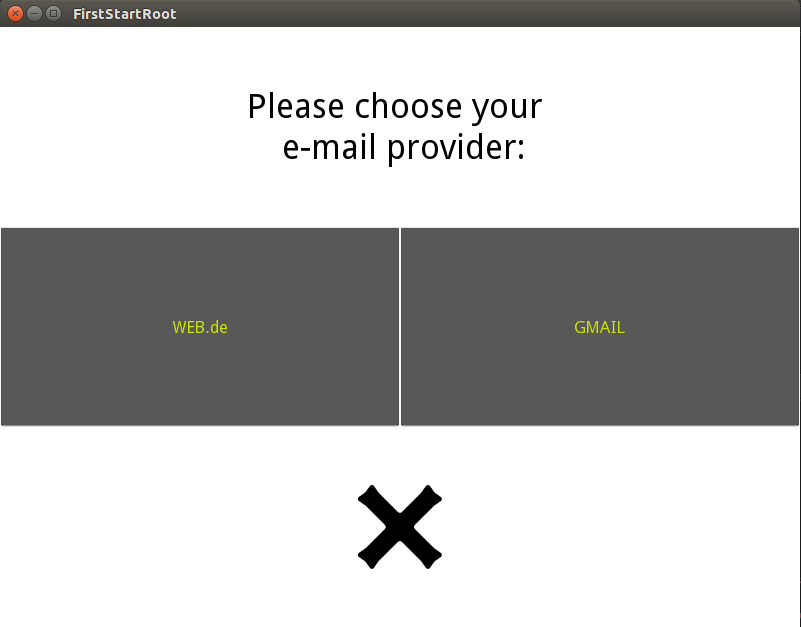
\includegraphics[scale=0.2]{Images/firstStartRoot.png}
%				\end{figure}
%		    	\end{frame}
%		
%			\begin{frame}
%				\frametitle{GUI}
%				\begin{figure}
%					\centering
%					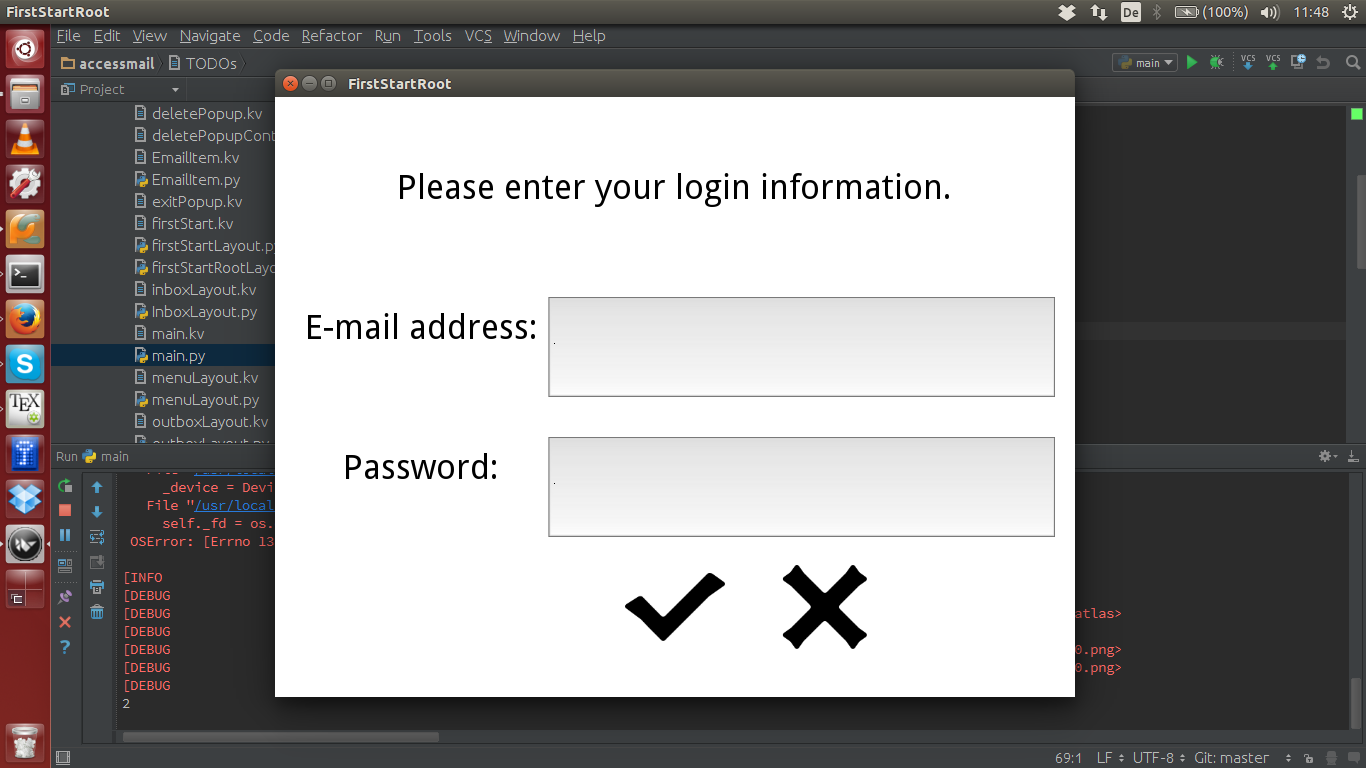
\includegraphics[scale=0.2]{Images/firstStartCredentials.png}
%				\end{figure}
%		    	\end{frame}
%			
%			\begin{frame}
%				\frametitle{GUI}
%				\begin{figure}
%					\centering
%					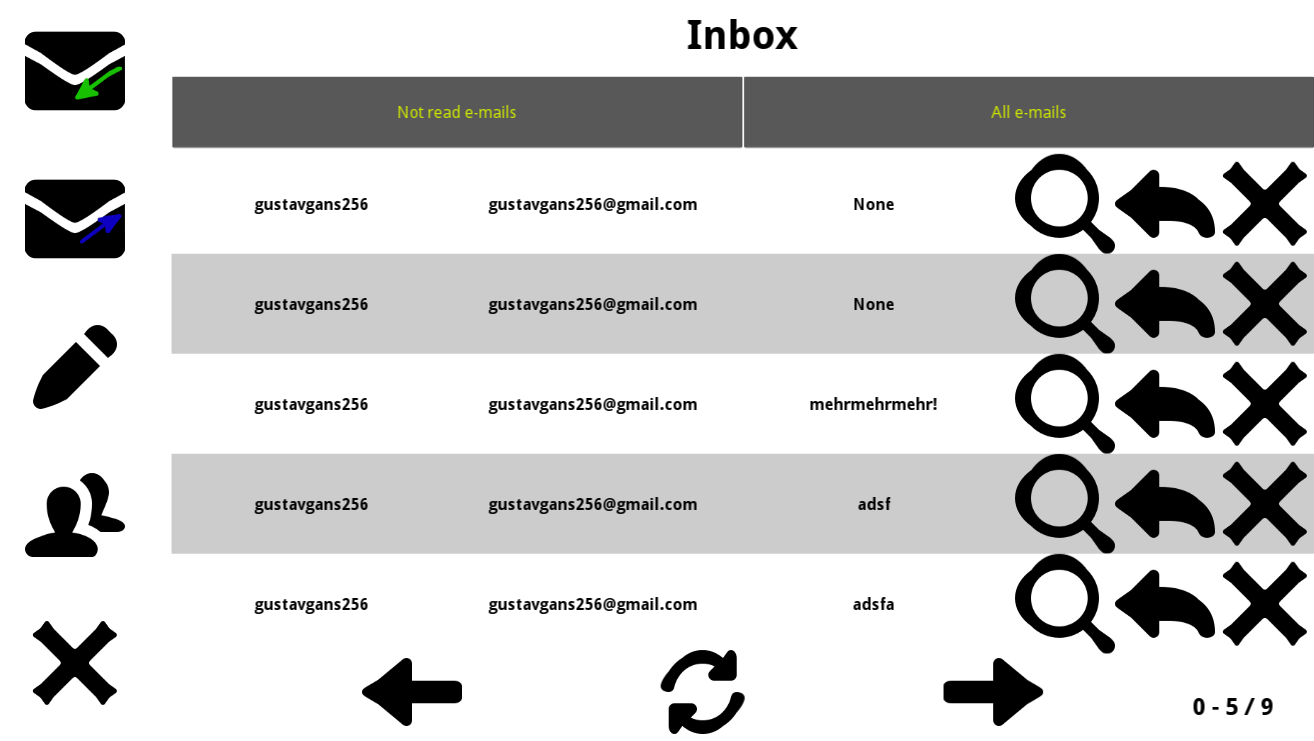
\includegraphics[scale=0.2]{Images/Inbox.png}
%				\end{figure}
%		    	\end{frame}
%			
%			\begin{frame}
%				\frametitle{GUI}
%				\begin{figure}
%					\centering
%					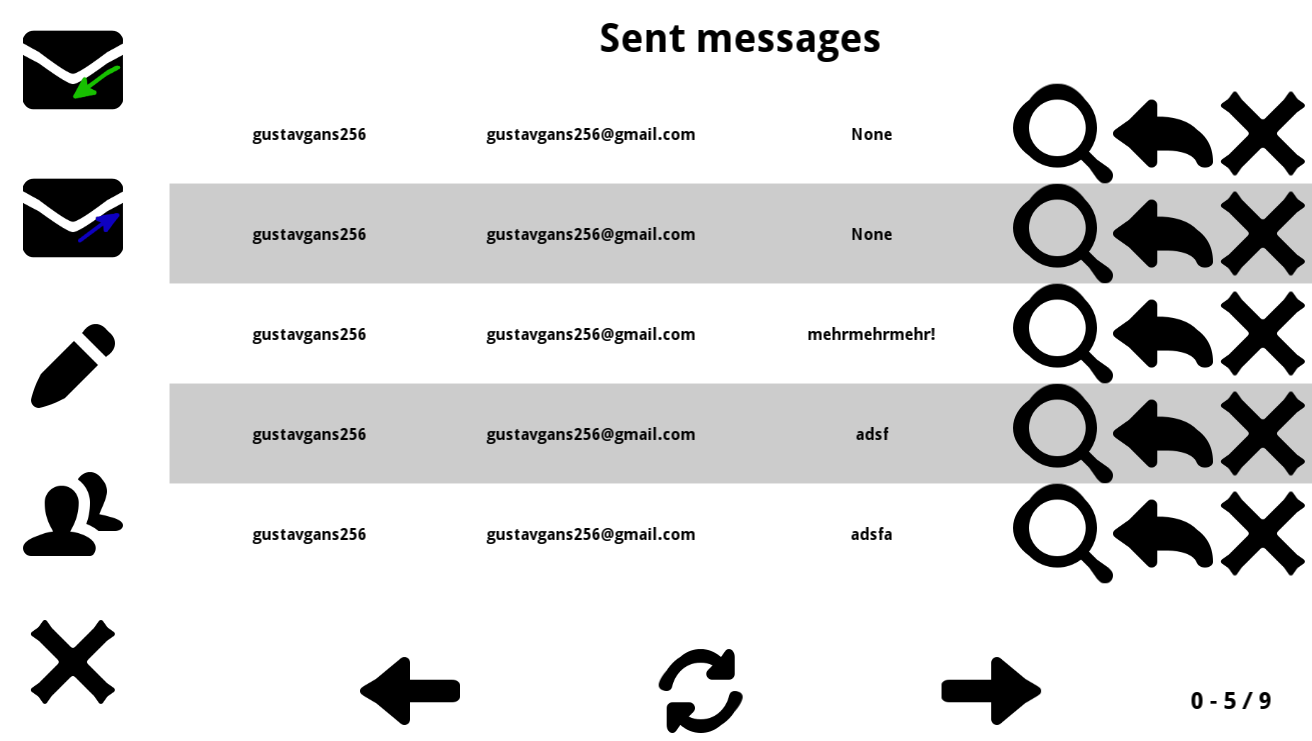
\includegraphics[scale=0.2]{Images/Outbox.png}
%				\end{figure}
%		    	\end{frame}
%		    	
%		    	\begin{frame}
%				\frametitle{GUI}
%				\begin{figure}
%					\centering
%					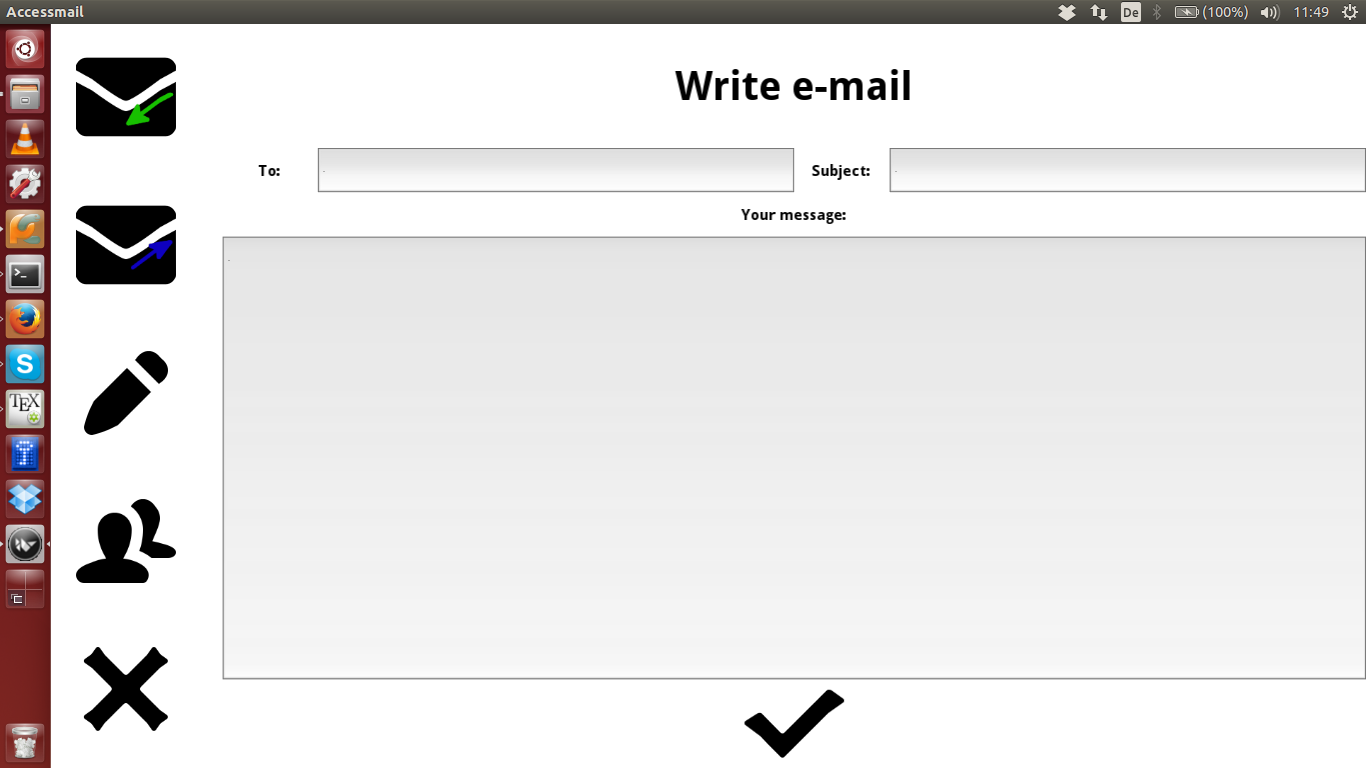
\includegraphics[scale=0.2]{Images/Write_blank.png}
%				\end{figure}
%		    	\end{frame}
%		    	
%		    	\begin{frame}
%				\frametitle{GUI}
%				\begin{figure}
%					\centering
%					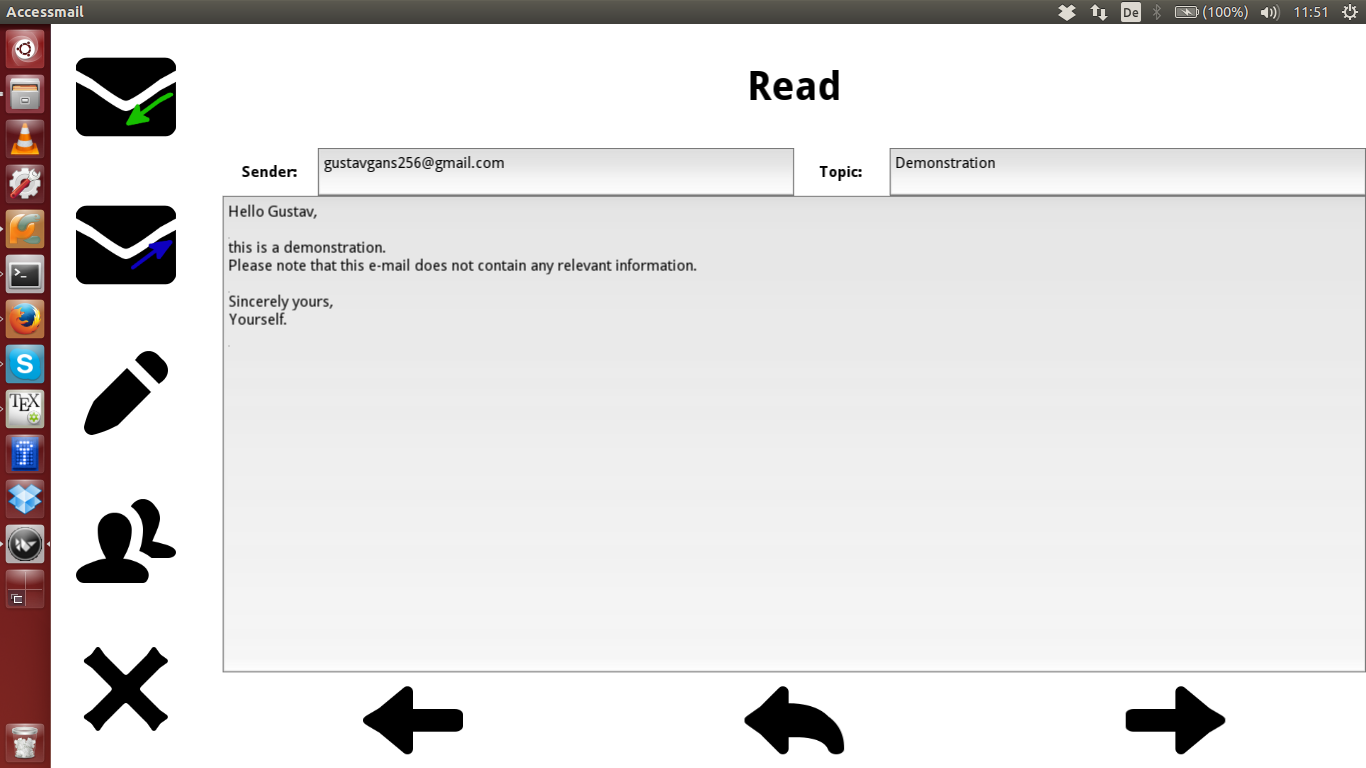
\includegraphics[scale=0.2]{Images/Read.png}
%				\end{figure}
%		    	\end{frame}
%		    	
%		    	\begin{frame}
%				\frametitle{GUI}
%				\begin{figure}
%					\centering
%					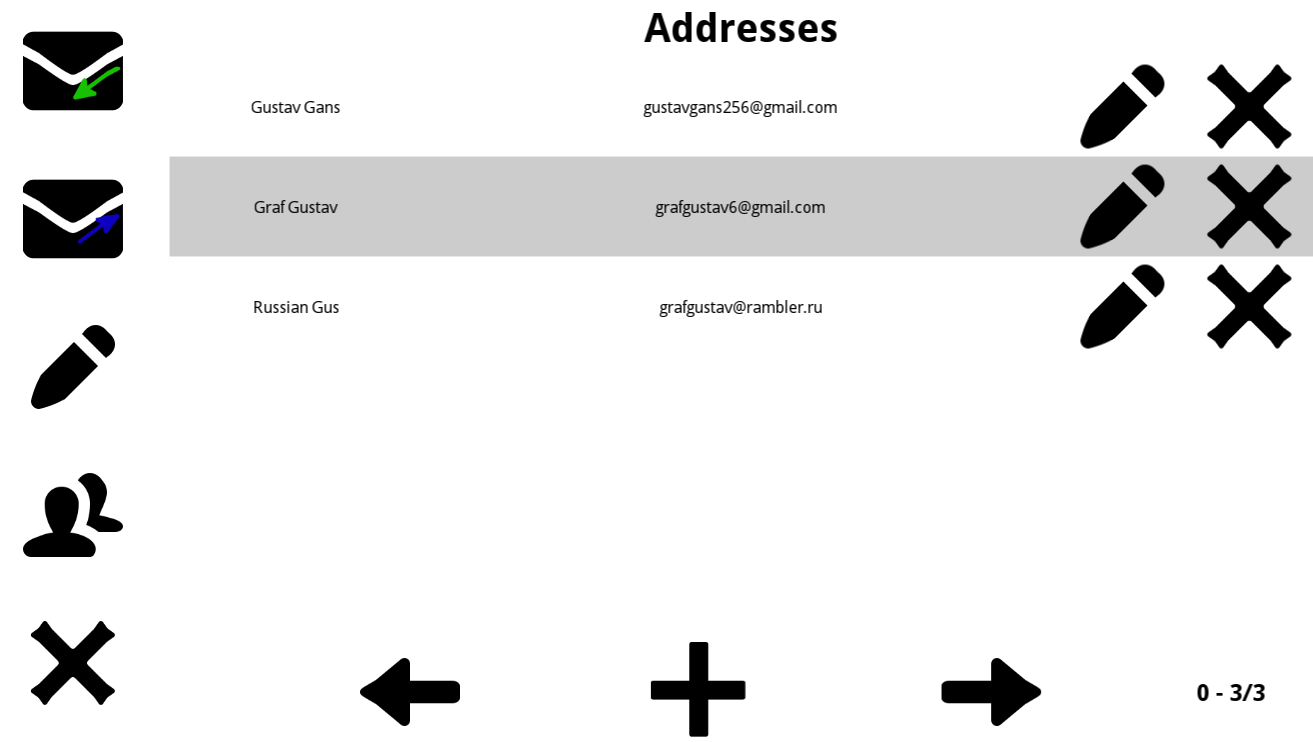
\includegraphics[scale=0.2]{Images/Addresses.png}
%				\end{figure}
%		    	\end{frame}
%		    	
%		    	\begin{frame}
%				\frametitle{GUI}
%				\begin{figure}
%					\centering
%					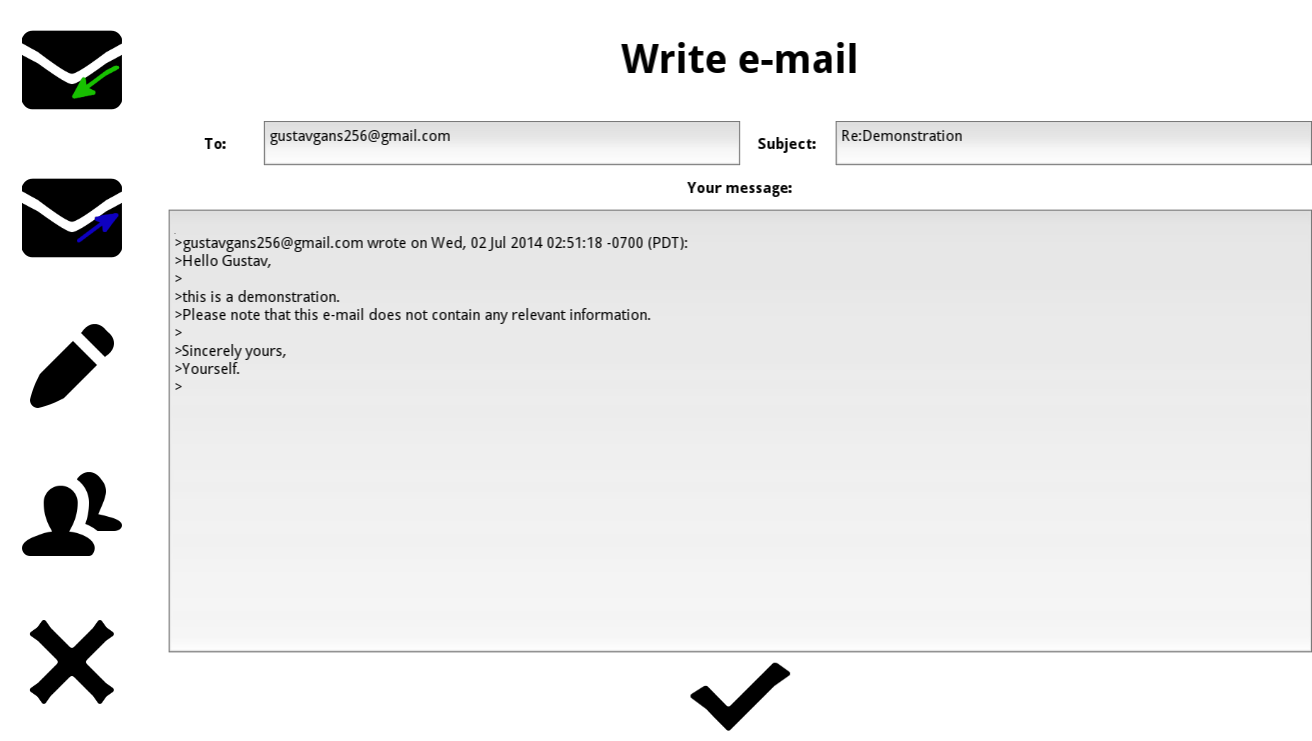
\includegraphics[scale=0.2]{Images/Answer.png}
%				\end{figure}
%		    	\end{frame}
%			\begin{frame}
%				\frametitle{Techniques}
%				
%		    	\end{frame}
		    	
	
	\section{Conclusion}
	
		\subsection{The software}
			\begin{frame}
				\begin{center}
					Let us have a look at the software!
				\end{center}
			\end{frame}
		
			\begin{frame}
				\frametitle{The software}
				%Diese Zusammenfassung ist nicht gut.
				\begin{itemize}
					\item Simple design
					\item High contrast
					\item No distractions
					\item Obvious pictographs
					\item Foreseeable behaviour
					\item Confirmations
				\end{itemize}
			
			\end{frame}
		
		\subsection{The future}
			\begin{frame}
				\frametitle{Future plans}
				%Diese Zusammenfassung ist nicht gut.
				\begin{itemize}
					\item More appealing design
					\item Photos to visualize contacts
					\item More language support
					\item Additional introduction (in simple language) for E-Mail
					\item More providers
					\item Completely keyboard accessible
				\end{itemize}
			
			\end{frame}

\end{document}
